\chapter{ESP32 Programmierung}

\section{Einführung (Becker, Specht)}

Die Programmierung der zeitkritischen Funktionalitäten erfolgt unter Verwendung eines \mbox{ESP-32}, da bestimmte Funktionen strengere zeitliche Anforderungen aufweisen, als dies mit einem General-Purpose-Betriebssystem realisierbar wäre.

Nach Abwägung aller relevanten Faktoren wurde sich dazu entschieden, den klassischen \mbox{ESP-32} Chip zu wählen, da dieser den Bluetooth Classic Standard unterstützt. 
Dieses Protokoll wird für die Ansteuerung des Dualshock4-Controllers benötigt.
Darüber hinaus trägt das weite Verbreitungsgebiet dieser Serie dazu bei, dass eine Vielzahl an Material zur Verfügung steht, was wiederum die Fehlersuche erheblich vereinfacht.

Es wurde jedoch ausdrücklich darauf verzichtet, den Controller unter Verwendung des Arduino Frameworks zu programmieren. 
Die Ursache hierfür war insbesondere die Größe der entstehenden Kompilate. 
Es sei darauf hingewiesen, dass das System über zahlreiche Funktionalitäten verfügt, was eine begrenzte Speicherverfügbarkeit zur Folge hat. 
Daher erfolgte die Programmierung des Controllers unter Verwendung des \textit{Espressif IoT Development Frameworks} (ESP-IDF) \cite{esp_esp_idf}. 
Dieses Framework stellt ebenfalls eine Vielzahl von Treibern für unterschiedliche Funktionen bereit, ist jedoch gezielt für Espressif-Controller konzipiert und zeichnet sich dadurch aus, dass es einen geringen Speicherplatzbedarf aufweist. 

Die Programmierung erfolgte in der Programmiersprache C.

\section{Motor-Treiber (Specht)}

Wesentlich für den Einstieg in die Motor-Treiber-Programmierung waren die verwendeten Hardware-Komponenten. Folgende Teile wurden verwendet:

\begin{itemize}
    \item 2x Pololu G2 High-Power Motor Driver 24v13 (MD31C)
    \item 2x MFA/Como Drills 919D501
\end{itemize}

Im ersten Ansatz wurde der Versuch unternommen, den Low-Level-Treiber (LL-Treiber) direkt mit der Differenzialantriebs-Logik (Differential Drive) zu koppeln. Nach intensiver Recherche und ersten Programmieransätzen wurde jedoch deutlich, dass eine klare Trennung beider Ebenen unter modularen Gesichtspunkten vorzuziehen ist. Diese Trennung resultiert in einer signifikanten Steigerung sowohl der Wiederverwendbarkeit als auch der Wartbarkeit des Codes. Abhilfe schafften hierbei vor allem die Verwendung von ESP-IDF-Komponenten.\newline

Um die Ansteuerung der Motoren zu realisieren, war es von zentraler Bedeutung, die Spezifikationen der verwendeten Hardware zu berücksichtigen. Das Datenblatt der Pololu-Motor-Treiber wurde in Form einer Webseite gefunden. Die darin enthaltenen Informationen waren ausreichend, um die Logik zu implementieren. Für die verwendeten Motoren lieferte das Datenblatt insbesondere elektrische Kenngrößen, die für die Absicherung der Hardware von entscheidender Bedeutung waren. Dazu zählten maximale und nominale Ströme. Zu Beginn des Projektes konnte nur auf einen 6V-Akku zurückgegriffen werden, obwohl die Motoren bis zu 12V-Betriebsspannung zulassen. Daraufhin wurden entsprechende Widerstände auf den Treiberboards angebracht, um den maximalen Strom für 6V zu begrenzen. Des Weiteren konnte aus dem Datenblatt des Pololu-Motor-Treibers die Notwendigkeit überdimensionierter Kondensatoren abgeleitet werden, um eine gute und stabile Performance sicherzustellen. \newline

Der Fokus der Implementierung lag vorrangig auf Modularität, Erweiterbarkeit, Clean-Code und Best-Practices. Dafür wurde wenn möglich auf globale Variablen verzichtet und stattdessen auf die Verwendung von Strukturen und Funktionen in Kombination mit Pointern gesetzt.

\subsection{Low-Level Treiber}

Die Aufgabe des LL-Treibers bestand darin, genau einen Motor anzusprechen und zu steuern. Das verwendete Framework ESP-IDF bietet eine Vielzahl an API-Funktionen, die eine abstrahierte und einfache Ansteuerung der Hardware ermöglichen. Für das Erzeugen von PWM-Signalen sind vor allem zwei API's von zentraler Bedeutung:

\begin{itemize}
    \item LED Control (LEDC)
    \item Motor Control Pulse Width Modulator (MCPWM)
\end{itemize}

Wie den Namen zu entnehmen ist, ist LEDC für die einfache Ansteuerung von LEDs gedacht, während MCPWM speziell für Motoren entwickelt wurde. Der MCPWM-Generator besteht aus einer Reihe von Submodulen, wie bspw. einem Fault-Module und einem Brake-Operator. Die Pololu-Boards bieten ebenfalls einen Fault-Pin, weshalb im weiteren Projektverlauf der MCPWM-Generator verwendet wurde, um diese Funktionalität nutzen zu können. \newline

Die MCPWM-API umfasst mehrere Funktionen und Strukturen. Deswegen wurde der erste Entwurf auf Basis einer Kombination aus KI-generierten Code und Beispielcode von Github erstellt. Die grundlegende Funktionalität konnte dadurch unkompliziert und schnell erfasst werden, wodurch Zeit gespart wurde. Nichtsdestotrotz war es notwendig, entsprechende Literatur zur API zu lesen und zu verstehen. Im Folgenden wurde der Code Stück für Stück angepasst, modularisiert und erweitert. \newline

Ein Key-Konzept entstand aus dem Gedanken, was passieren würde, wenn ein Duty-Cycle von beispielsweise 100 \% (Volllast) gesetzt wird und die Drehrichtung des Motors umgekehrt wird. Die Annahme war, dass der Motor in diesem Fall solange als Generator arbeitet, bis die Richtung letztendlich umgekehrt wird. Der dabei möglicherweise auftretende Rückstrom könnte eventuell die Hardware beschädigen. Aus diesem Grund wurde sich auf eine Ramping-Strategie geeinigt, die eine sichere und kontrollierte Änderung der Drehrichtung ermöglicht. Dabei soll sichergestellt werden, dass der Duty-Cycle des PWM-Signals bzw. die Richtung für den Motor nicht abrupt geändert wird. Stattdessen wird der Duty-Cycle in konfigurierbaren Schritten dem Nullbereich angenähert. In einem sicheren Hysteresebereich wird dann die Richtung geändert und der Duty-Cycle der neuen gewünschten Geschwindigkeit angepasst. \newline

Ein weiterer wichtiger Baustein sollte das automatisierte Erkennen von Fehlern der Motoren sein. In solch einem Fall sollte der Motor sofort gestoppt werden und eine Signalleuchte angehen. Ein einfacher Testaufbau bestehend aus Pull-up Widerständen und einer LED sollte die grundlegende Funktionalität des Fault-Pins sicherstellen.

\begin{figure}[h]
    \centering
    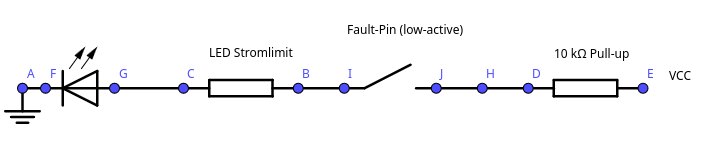
\includegraphics[width=\textwidth]{images/motor_driver_fault_pin.png}
    \caption{Testaufbau des Fault-Pins des Pololu-Motor-Treibers}
    \label{fig:motor_driver_fault_pin}
\end{figure}

Der Fault-Pin ist laut Datenblatt ein Open-Drain-Ausgang, der bei einem Fehler auf Low gezogen wird. Im Testaufbau wurde ein Pull-Up-Widerstand von 10 k$\Omega$ verwendet, um den Pin im Normalfall auf High zu halten. Folgendes Verhalten wurde erwartet: Bei einem Fehler wird der Pin auf Low gezogen und die LED leuchtet auf. Dies war jedoch nicht der Fall. Stattdessen leuchtete die LED dauerhaft, obwohl der Motor einwandfrei funktionierte. Nach Rücksprache mit dem Betreuer stellte sich heraus, dass dieser Pin in der Vergangenheit nie benutzt wurde. Um den Projektfortschritt nicht unnötig zu gefährden, wurde beschlossen, den Fault-Pin nicht weiter zu verwenden und mit der Implementierung des Differential Drive fortzufahren.

\subsection{Low-Level Treiber Test}

Das Testing wurde in mehreren Schritten durchgeführt. Für die Erstellung der Testfälle wurde dabei zum Großteil KI-generierter Code verwendet. Dadurch konnte der damit verbundene Zeitaufwand signifikant minimiert und zugleich eine minimale Testabdeckung garantiert werden. \newline

Zunächst sollte die grundlegende Funktionalität des LL-Treibers getestet werden. Dazu wurden LEDs auf einem Breadboard angebracht, welche die Motoren simulieren sollten. Die Helligkeit der LEDs sollte dabei die Geschwindigkeit des Motors repräsentieren. \newline

Nach erfolgreicher Validierung der Ergebnisse wurde der Testaufbau an die echte Hardware angepasst. Zudem sollte ein Wrapper erstellt werden, der beide Motoren über einzelne Treiber-Objekte anspricht. Dies stellte somit eine Vorstufe zum Differential Drive dar. Ziel war es, die beiden Motoren unabhängig voneinander ansteuern zu können. Dafür wurde das Fahrzeug auf einer Holzkonstruktion bestehend aus zwei Holzlatten platziert. Obwohl die Tests positiv verliefen, sollte sich der Test ohne Bodenkontakt im weiteren Projektverlauf als suboptimal herausstellen.

\subsection{Differential Drive}



\subsection{Tests}

\subsection{Integration}

\section{MQTT-Anbindung (Specht)}

\subsection{WiFi-Stack}

\subsection{MQTT-Stack}

